%\documentclass[ignorenonframetext]{beamer}

\documentclass[fleqn,
  11pt, %default: 11pt
  xcolor=dvipsnames, 
  aspectratio=1610, 
  ]{beamer}% 11pt is default
% Possible values for aspectratio are: 169 (160mm by 90mm), 1610 (160mm x 100mm), 149, 54, 43 (128mm by 96mm, default), 32.

\usepackage{etex} % to avoid error "No room for a new \dimen" when loading the decorations tikzlibrary
\usepackage[absolute,overlay]{textpos}


\usepackage{amsthm} %for theorem environments
\usepackage{amssymb} %lots of math symbols
\usepackage{mathtools} %for, e.g., \DeclareMathOperator
\usepackage{amsmath} %for spacing in equations and aligns
\usepackage{mathbbol} %for \1, load at last
\usepackage{mathrsfs}
\usepackage{amsfonts} 
\usepackage{marvosym}% for \Lightning and \RightScissors

\usepackage{pifont}
\usepackage{lmodern}%to avoid font size warnings

\usepackage{graphicx}
\graphicspath{{../pics/}}
\usepackage{listings}
\usepackage{array}
\usepackage{makecell}
\usepackage{mathtools}
% \usepackage{complexity}
% \newlang{\TSP}{TSP}
\usepackage{calc}%for \widthof{text}
\usepackage{multicol}
\usepackage{booktabs}
%\usepackage{enumitem}

% show numbers in the bibliography
\setbeamertemplate{bibliography item}[text]
%\setbeamertemplate{page number in head/foot}{}

% print emphasized text in structure color instead of italic in beamer mode
\renewcommand{\emph}[1]{\structure{#1}}
\newcommand{\gruen}[1]{{\color{NiceGreen} #1}}
\newcommand{\dunkelrot}[1]{{\color{DarkRed} #1}}
\newcommand{\rot}[1]{{\color{red} #1}}
\newcommand{\LG}[1]{{\color{lightGray} #1}}
\newcommand{\grau}[1]{{\color{black!60} #1}}

% restrict equation numbering to referenced equations in beamer mode
\mathtoolsset{showonlyrefs}

%disable navigation symbols
\setbeamertemplate{navigation symbols}{}

%document setup
\usepackage[utf8]{inputenc} 

%language setup
\usepackage[english]{babel}

%color and picture modification packages 
%\usepackage{colortbl}
\usepackage{fix-cm}
\usepackage{multirow}
\usepackage{setspace}
\usepackage{multicol}
\usepackage{ifthen}% iftheles
%%% ---------------------- TikZ -------------------------
\usepackage{pgfplots}
\pgfplotsset{compat=newest}
\usepackage{tikz}
\usepackage{qrcode}
\usetikzlibrary{
  % shapes,
  shapes.geometric,
  shapes.arrows,
  % chains,
  % decorations.pathreplacing,
  decorations.pathmorphing,
  decorations.markings, % can mess up the axes for pgfplots
  positioning,
  fit,
  fadings,
%   backgrounds,
  calc,
  shapes.callouts,
  patterns, 
  fillbetween,
  }

\newcommand{\rndpos}{\pgfmathparse{0.2}\pgfmathresult}

% red bullets in itemize with <red@1->
\newenvironment{redenv}{\only{\setbeamercolor{local structure}{fg=red}}}{} 
\newenvironment{defaultenv}{\only{\setbeamercolor{local structure}{fg=niceblue}}}{} 

%own themes
\useoutertheme[nofootline]{wuerzburg}
\usecolortheme{shark}
\useinnertheme[realshadow,corners=2pt,padding=2pt]{chamfered}
\usefonttheme{professionalfonts}

%custom colors
\setbeamercolor{black}{bg=black}

\definecolor{DarkGray}{gray}{0.25} 
\definecolor{MidGray}{gray}{0.38} 
\definecolor{NeutralGray}{gray}{0.5}
\definecolor{LightGray}{gray}{0.7}
\definecolor{lightGray}{gray}{0.85}
\definecolor{DarkRed}{rgb}{0.7,0,0}
\definecolor{DarkBlue}{rgb}{0,0,0.5}
\definecolor{SteelBlue}{rgb}{0,0.4,0.6}
\definecolor{Orange}{rgb}{0.7,0.5,0}
\definecolor{Violette}{rgb}{0.5,0,0.5}
\definecolor{Sand}{rgb}{0.84,0.8,0.55}
\definecolor{niceblue}{rgb}{0.33,0.5,0.8}
\definecolor{OliveGreen}{RGB}{0,102,102}
\definecolor{NiceGreen}{RGB}{0,153,72}

%other
\newcommand{\cmark}{\ding{52}}
\newcommand{\xmark}{\ding{55}}

\newcommand{\tikzframe}[2]{
	\begin{frame}[t]\frametitle{#1}
		\begin{tikzpicture}[ol]
		#2
		\end{tikzpicture}
	\end{frame}	
}

\newcommand{\specialcell}[2][c]{%for cells in tabulars
  \begin{tabular}[#1]{@{}c@{}}#2\end{tabular}}

% set itemsep in itemize, enumerate, ...
\newcommand{\MyItemSep}[1]{\setlength\itemsep{#1 \baselineskip}} 

\newcommand{\myBlock}[3][0.6]{
  \begin{minipage}{#1 \linewidth}
  \begin{block}{#2}
  #3
  \end{block}
  \end{minipage}
}

\newenvironment{MRuleBlock}[3]{%
\begin{minipage}[t][#2][t]{#3}%
\begin{block}{#1}%
}{%
\end{block}%
\end{minipage}%
}

\renewcommand{\mp}[3][]{%
  #1%
  \begin{minipage}{#2\linewidth}%
    #3%
  \end{minipage}%
  % \flushleft%
  }



\newcommand{\fs}[1]{{\footnotesize #1}}
\newcommand{\sms}[1]{{\small #1}}
\newcommand{\fos}[1]{{\footnotesize #1}}
\newcommand{\scs}[1]{{\scriptsize #1}}
\newcommand{\tis}[1]{{\tiny #1}}



\newcommand<>{\PutAt}[3][0pt]{%
    {\only#4{\begin{textblock*}{#1}#2%
      #3
    \end{textblock*}}}%
  }

\newcommand{\To}{$\to$}
\newtheorem{conjecture}{Conjecture}

%%% ============= meta data ================
\title
	[Klassifizierung von CitiBike-Kunden]
	{Klassifizierung von CitiBike-Kunden}
	
\date{}

\author{Thomas Wagner}

\hypersetup{
  pdfauthor={Thomas Wagner},
  pdftitle={AXA Data Science Challenge},
  pdfsubject={},
  pdfproducer={latex beamer}
}

%\usepackage{nicematrix}
%\usepackage{tikz}
\usetikzlibrary{matrix}

\definecolor{highlightred}{RGB}{168,59,0}
\newcommand<>{\highlight}[1]{\textcolor#2{highlightred}{#1}}

\newcommand{\Conv}{\mathop{\scalebox{1.5}{\raisebox{-0.2ex}{$\ast$}}}}
\newcommand{\stab}{\mathfrak{S}}
\DeclareMathOperator{\argmax}{argmax}

%=====================================================

%%% =============== begin document =====================
\begin{document}

\setlength\mathindent{1em}
%
\begin{frame}[t]\frametitle{}
	\titlepage
\end{frame}

\begin{frame}{Agenda}
\centering
\myBlock[0.6]{}
{
\begin{enumerate}
\item \highlight{Projektbeschreibung}
\item Datenset und Features
\item Feature-Visualisierung
\item Modell-Training und -Auswahl
\item Kooperationsmöglichkeiten mit einer Versicherung
\end{enumerate}
}
\end{frame}

\section{Projektbeschreibung}

\begin{frame}{CitiBike}
\begin{columns}
\begin{column}{0.4\linewidth}
%\emph{CitiBike-Stationen (2022)}\\[.2cm]
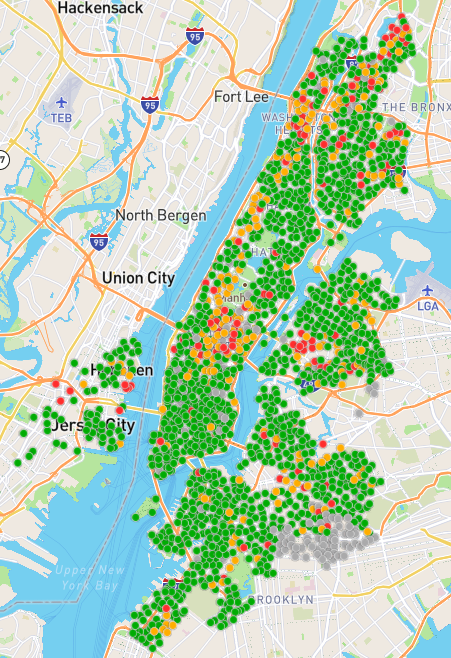
\includegraphics[height=0.9\textheight]{Bilder/CitiBike-Map.png}
\end{column}
\begin{column}{0.6\linewidth}

%\only<1>
%{
\myBlock[1]{CitiBike in 2022}
{
\begin{itemize}
\item über 24.000 Fahrräder
\item über 1.500 Verleihstationen
%\item über 17 Millionen Fahrten
\end{itemize}
}
%}
\myBlock[1]{Subscription-Modell}
{
\begin{itemize}
\item \highlight{Subscriber}:
\begin{itemize}
\item  Jährliche Mitgliedschaft (15 \$ / Monat)
\end{itemize}
\item \highlight{Customer}: 
\begin{itemize}
\item \makebox[0.7cm][r]{4 \$} einfache Fahrt
\item \makebox[0.7cm][r]{15 \$} Tagespass
\end{itemize}
\end{itemize}
}
{\PutAt<2>[10cm]{(3cm,4.5cm)}{\myBlock[1]{\LARGE Projekt}{\Large Nutzer-Klassifizierung (Customer/Subscriber)}}}
\end{column}
\end{columns}
\end{frame}

\begin{frame}{Datensatz}
\myBlock[1]{Daten von 2018}{17 Millionen Fahrten,  800 			Stationen, 15.000 Fahrräder
	}

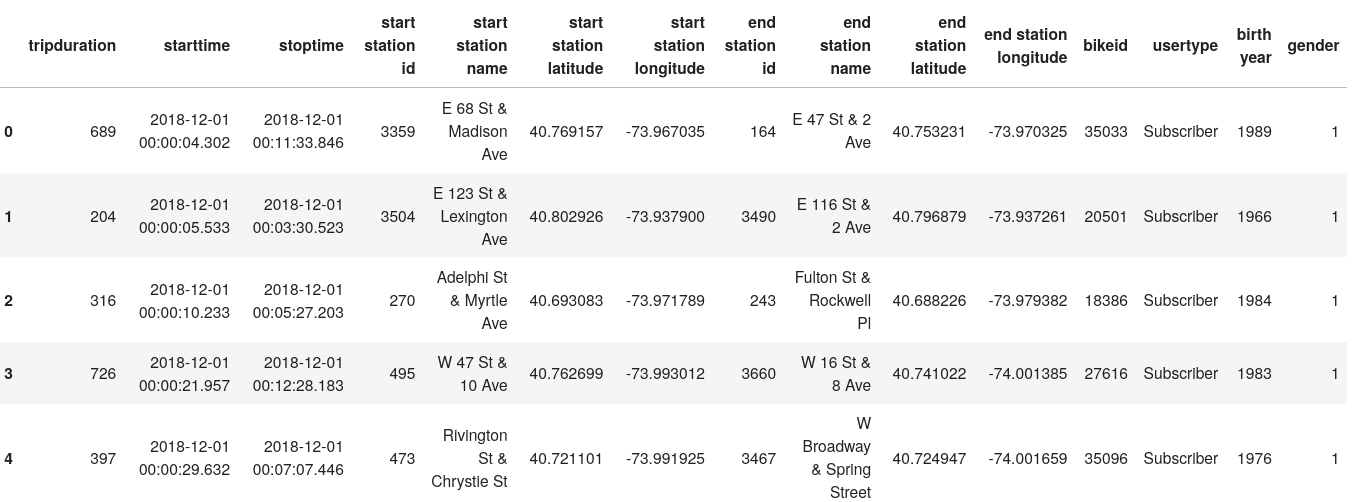
\includegraphics[width = \textwidth]{Bilder/Data}

\only{\tiny{Gender: 0 = unknown, 1 = male, 2 = female \; Tripduration: in Sekunden}}
\end{frame}




\begin{frame}{Vorgehen und Tools}
\begin{columns}
\begin{column}{0.5\textwidth}
\begin{MRuleBlock}{Vorgehen}{3.45cm}{\textwidth}
\begin{enumerate}
\item Daten \highlight<1>{laden} und \highlight<1>{formatieren}
\item Daten \highlight<2>{säubern}
\item Daten \highlight<3>{analysieren} und \highlight<3>{visualisieren}
\item Modelle \highlight<4>{trainieren} und \highlight<4>{auswählen}
\end{enumerate}
\end{MRuleBlock}
\end{column}
\begin{column}{0.5\textwidth }
\centering
\begin{MRuleBlock}{Tools}{3.45cm}{\textwidth}
\vspace{0.5\baselineskip}
\begin{itemize}
\item \highlight<1-2>{Pandas}
\item \highlight<3>{Matplotlib}, \highlight<3>{Seaborn}
\item \highlight<4>{Scikit-Learn}
\end{itemize}
\vspace{0.3\baselineskip}
\end{MRuleBlock}
\end{column}
\end{columns}
\end{frame}


\begin{frame}{Agenda}
\centering
\myBlock[0.6]{}
{
\begin{enumerate}
\item Projektbeschreibung
\item \highlight{Datenset und Features}
\item Feature Visualisierung
\item Modell Training und Auswahl
\item Kooperationsmöglichkeiten mit einer Versicherung
\end{enumerate}
}
\end{frame}
%\begin{frame}
%\begin{beamercolorbox}[sep=8pt,center]{title}
%    \usebeamerfont{title}{Datenset und Features}
%\end{beamercolorbox}
%\end{frame}

\section{Datenset und Features}

\begin{frame}{Data-Loading}
\myBlock[1]{Daten-Format}
{
\begin{itemize}
\item Eine CSV-Datei pro Monat.
\item Naives Einlesen benötigt $>$ 9 GB Speicher.
\end{itemize}
}
\myBlock[1]{Daten-Konvertierung}
{
\begin{itemize}
\item Pandas \highlight{Category-dtype} für Stationsnamen.
\item Pandas \highlight{Datetime-dtype} für Timestamps.
\item Zusammenführen von Kategorien über mehrere Dateien.
\item Parquet-Format zum Erhalt von dtype-Information.
\end{itemize}
}
\end{frame}

%\begin{frame}
%\begin{beamercolorbox}[sep=8pt,center]{title}
%    \usebeamerfont{title}{Wichtige Features}
%\end{beamercolorbox}
%\end{frame}

\begin{frame}{Wichtige Features}
\myBlock[0.48]{Fahrtdauer}
{
\centering
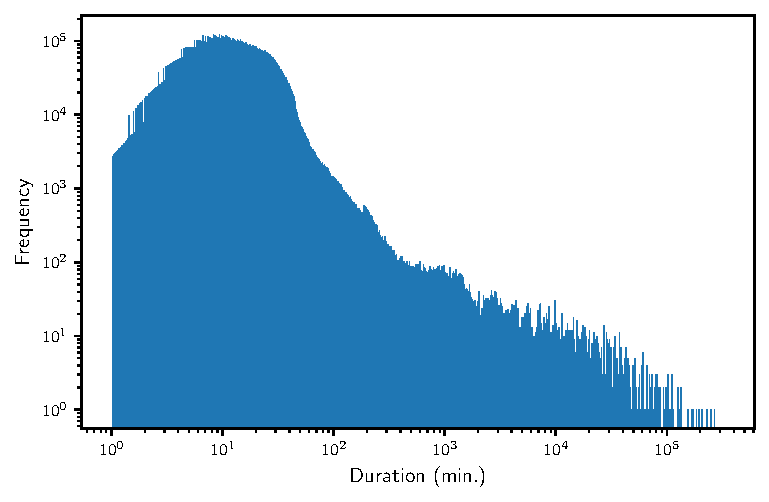
\includegraphics[width=0.9\textwidth]{../Images/Tripduration}
\begin{itemize}
\item<1> Typische Fahrten zwischen 2-60 min.
\item<1> Fahrten kürzer als 1 min. von CitiBike entfernt.
\item<1> 350.000 Rundfahrten

(Startstation = Endstation)
\end{itemize}
}
\myBlock[0.48]{Haversine-Distanz}
{
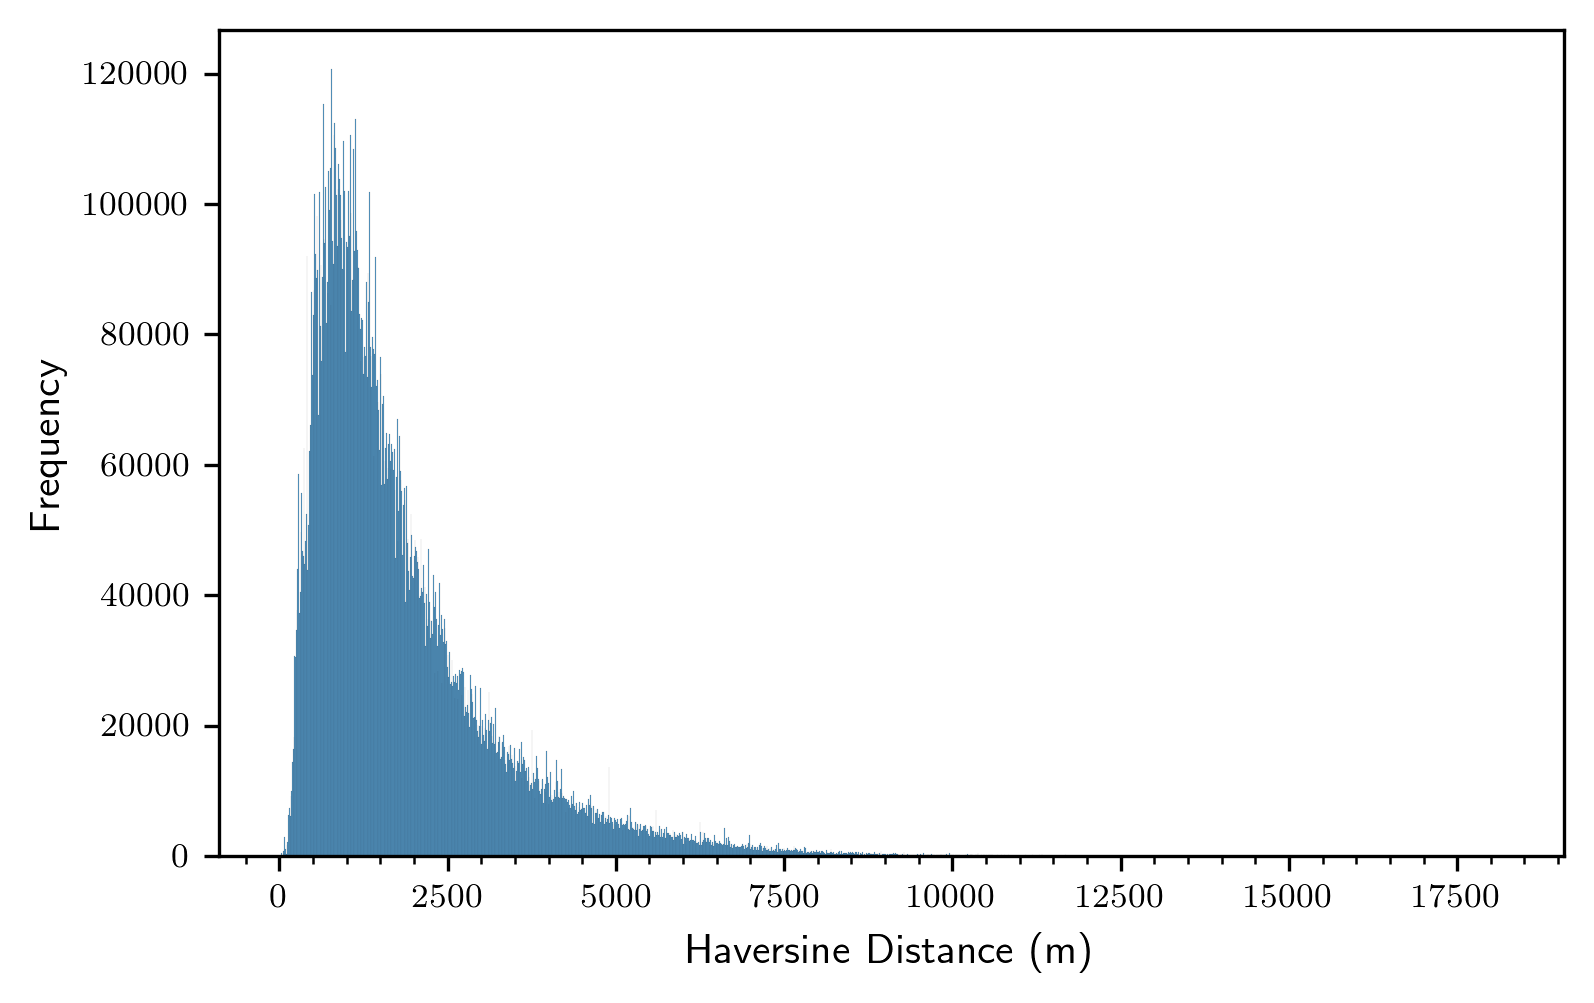
\includegraphics[width=0.9\textwidth]{../Images/Distance.png}
\begin{itemize}
\item Luftlinie Start- zu End-Koordianten
\item Keine Routen Information
\item \highlight{Geschwindigkeit} =

 Distanz / Fahrtdauer
\item 0 für Rundfahrten
\end{itemize}
}
\end{frame}

\begin{frame}{Wichtige Features}
\myBlock[0.48]{Jahreszeit}
{
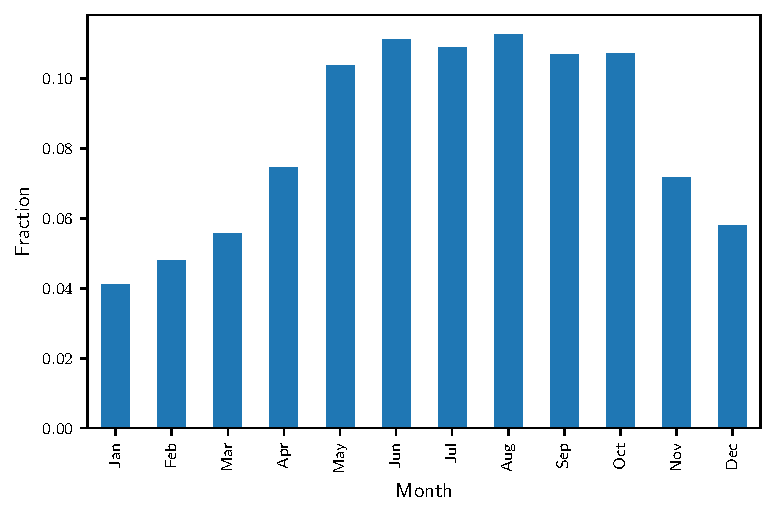
\includegraphics[width=0.9\textwidth]{../Images/CountByMonth}
\begin{itemize}
\item Mehr Fahrten zwischen Mai und Oktober
\item Kategorisierung in "Sommer" und "Winter"
\end{itemize}
}
\myBlock[0.48]{Werktage}
{
\centering
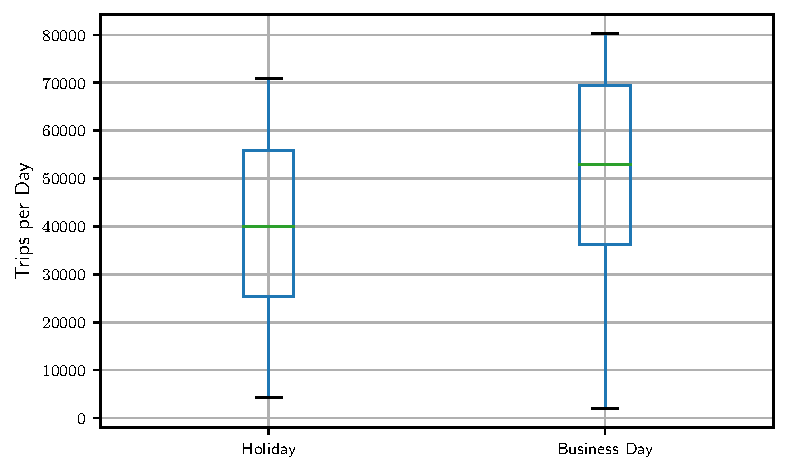
\includegraphics[width=\textwidth]{../Images/CountByBusiness}
\begin{itemize}
\item 251 Werktage
\item 114 Ferientage / Wochenenden
\end{itemize}
}
\end{frame}

\begin{frame}{Nicht-Balancierte Daten}
\centering
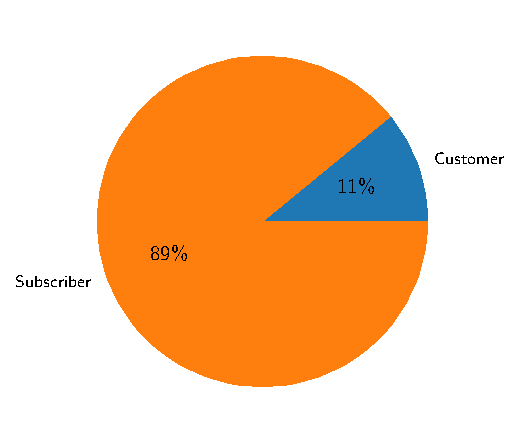
\includegraphics[height=0.9\textheight]{../Images/Piechart}
\end{frame}

\begin{frame}{Data Cleaning}
\centering
\myBlock[0.6]{Entferne: }
{
\begin{itemize}
\item 3000 Einträge: fehlenden Station IDs.
\item 11.000 Einträge: geboren vor 1920.
\item 65 Einträge: Latitude $ > 45$ (Montreal?).
\item 175 Einträge: Geschwindigkeit $ > 40$ km/h.
\item 15.000 Einträge: länger als 5 h
\item 40.000 Einträge: Rundfahrt unter 2 min.
\end{itemize}
}
%\end{column}
%\end{columns}
\end{frame}

\begin{frame}{Training-Test Split}

\myBlock[1]{Validationset oder Kreuzvalidierung?}
{
\begin{itemize}
\item Kreuzvalidierung:
\begin{itemize}
\item K-facher Split des Datensets
\item K-Modelle: Training auf (K-1)-Teilen, Test auf einem Teil
\item Ermöglicht Nutzung von mehr Trainings Daten
\item Rechenzeit aufwendiger
\end{itemize}
\item Hier:
\begin{itemize}
\item Mehr als 17 Millionen Datenpunkte.
\item $80\%-10\%-10\%$ Training-Validation-Test Split.
\item SE auf der kleineren Klasse $\approx \pm 0.02\%$ (bei einer Genauigkeit von $99\%$).
\end{itemize}
\highlight{Keine Kreuzvalidierung nötig.}
\end{itemize}
}
\end{frame}

\begin{frame}
\centering
\myBlock[0.7]{Zusammenfassung}
{
\begin{itemize}
\item Bisher:
\begin{itemize}
\item Betrachtung des gesamten Datensets
\item Erste Identifikation von Features
\item Keine Betrachtung von Labels
\end{itemize}
\item Nächster Schritt:
\begin{itemize}
\item Betrachtung der Labels (nur auf Trainingset)
\item Auswahl sinnvoller Features.
\end{itemize}
\end{itemize}
}
\end{frame}

\section{Feature Visualisierung}

\begin{frame}{Agenda}
\centering
\myBlock[0.6]{}
{
\begin{enumerate}
\item Projektbeschreibung
\item Datenset und Features
\item \highlight{Feature Visualisierung}
\item Modell Training und Auswahl
\item Kooperationsmöglichkeiten mit einer Versicherung
\end{enumerate}
}
\end{frame}

\begin{frame}{Jahreszeit und Ferien}
\begin{columns}
\begin{column}{0.5\linewidth }
\centering
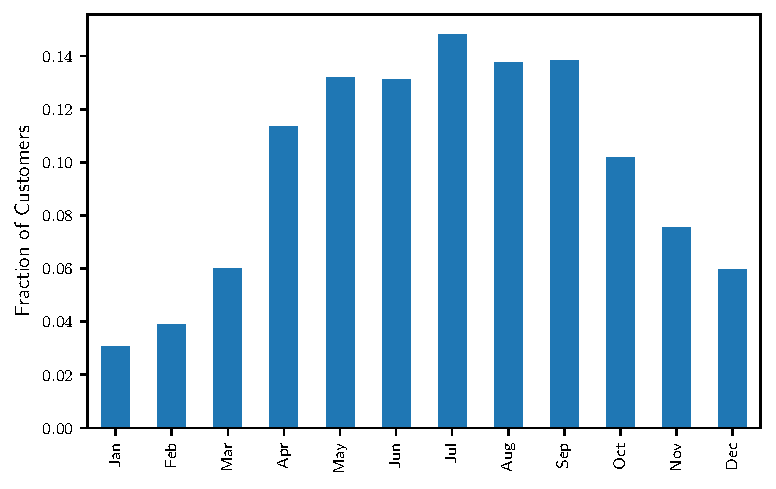
\includegraphics[width=\linewidth]{../Images/CountByMonthCustomers}
\end{column}
\begin{column}{0.5\linewidth }
\centering
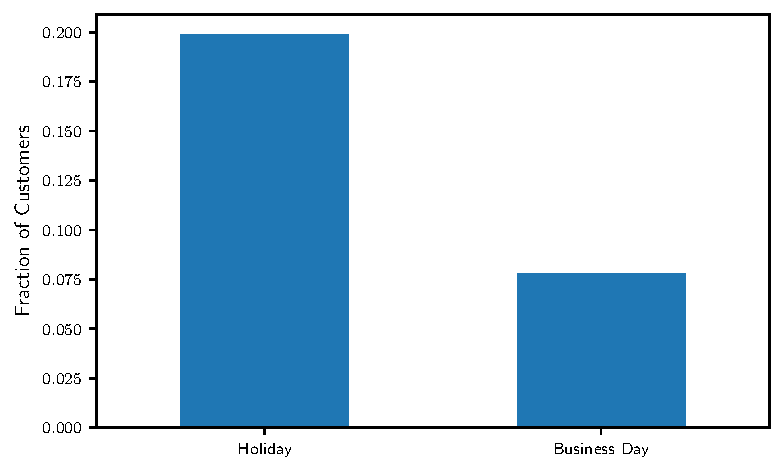
\includegraphics[width=\linewidth]{../Images/CountByBusinessCustomers}
\end{column}
\end{columns}

\myBlock[1]{Zusammenfassung}
{
Customer fahren häufiger:
\begin{itemize}
\item im Sommer.
\item an Feiertagen und Wochenenden.
\item Kategorisierte Features.
\end{itemize}
}
\end{frame}

\begin{frame}{Distanz und Geschwindigkeit}
\begin{columns}
\begin{column}{0.5\linewidth }
\centering
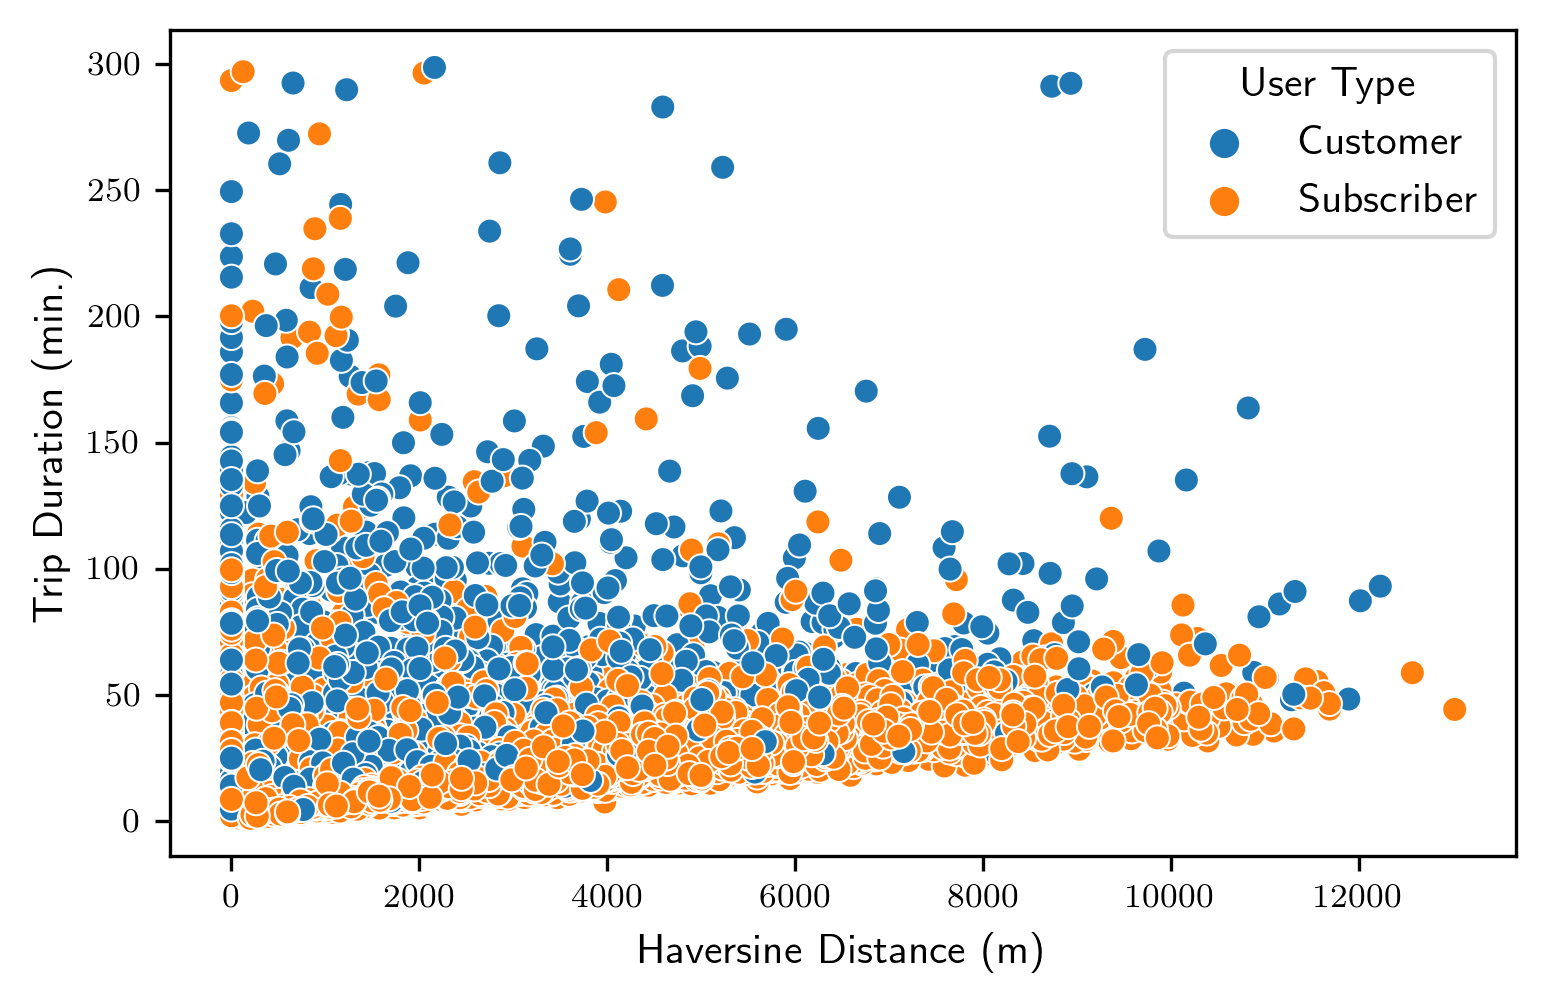
\includegraphics[height=0.45\textheight]{../Images/TimeVsDistance}
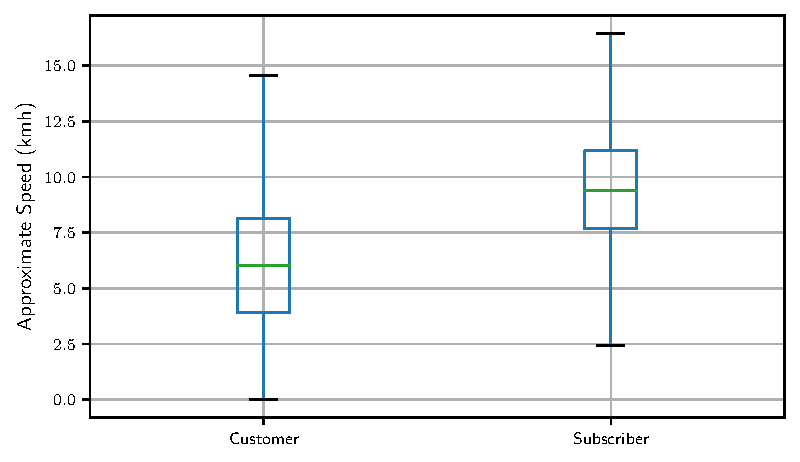
\includegraphics[height=0.45\textheight]{../Images/SpeedComparison}
\end{column}
\begin{column}{0.5\linewidth }
\centering
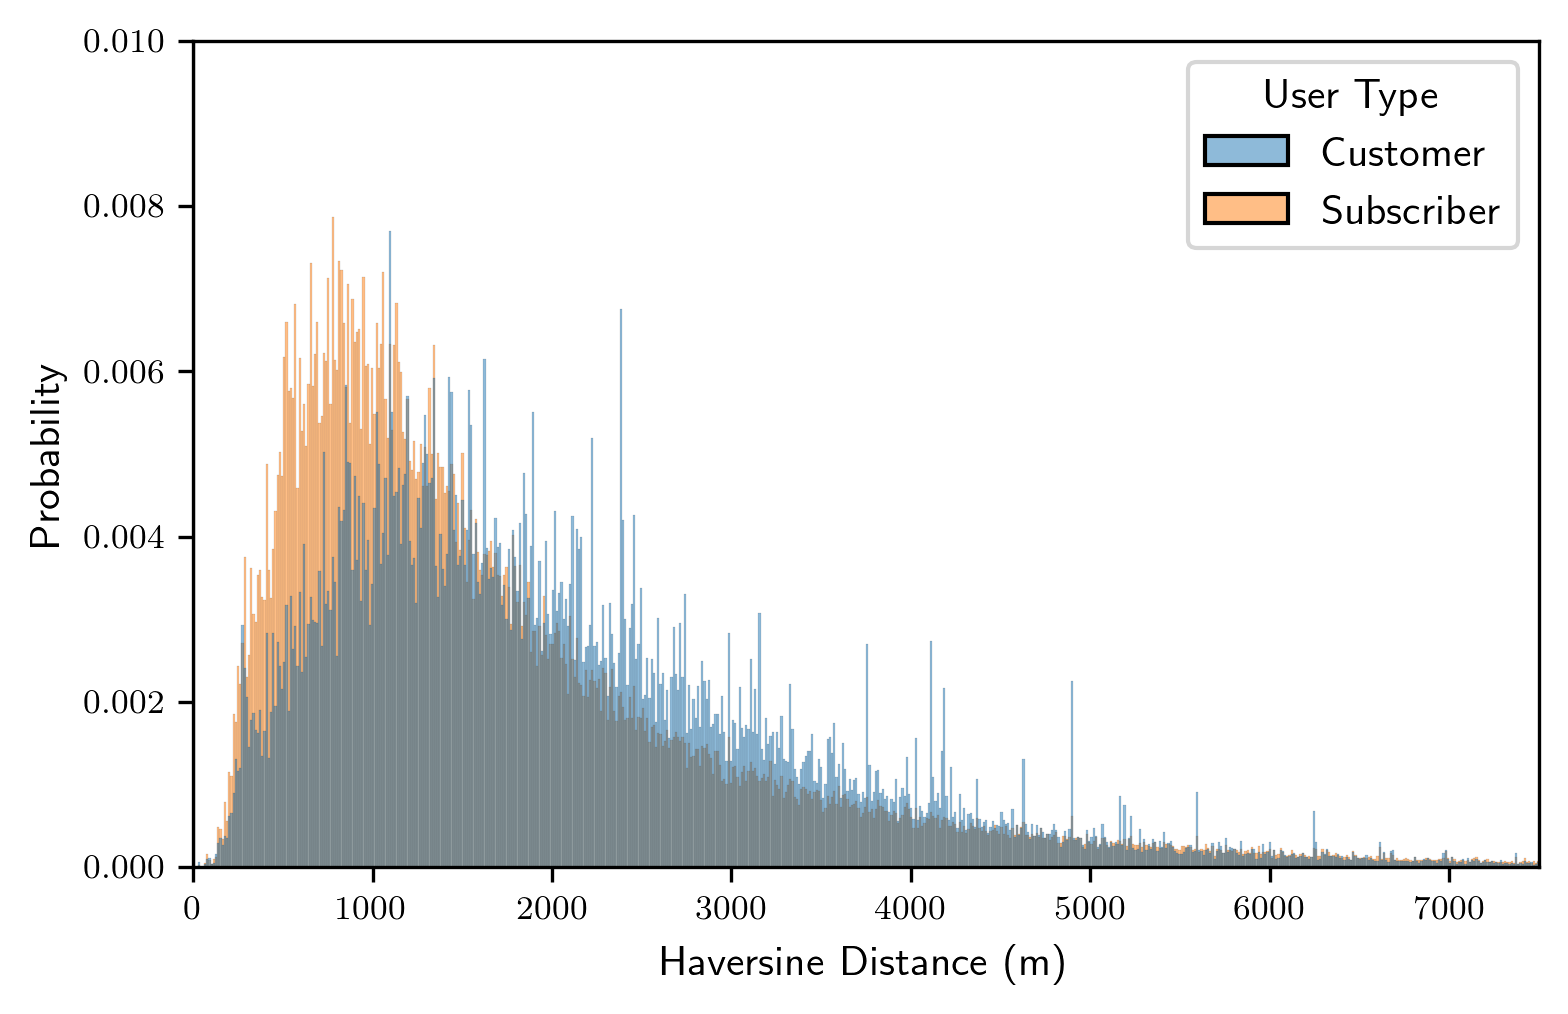
\includegraphics[height=0.45\textheight]{../Images/DistanceComparison}
\myBlock[1]{Zusammenfassung}
{
Customer machen:
\begin{itemize}
\item mehr Rundfahrten.
\item langsamere Fahrten.
\item etwas längere Fahrten.
\end{itemize}
}
\end{column}
\end{columns}
\end{frame}

\begin{frame}{Start Zeit}
\centering
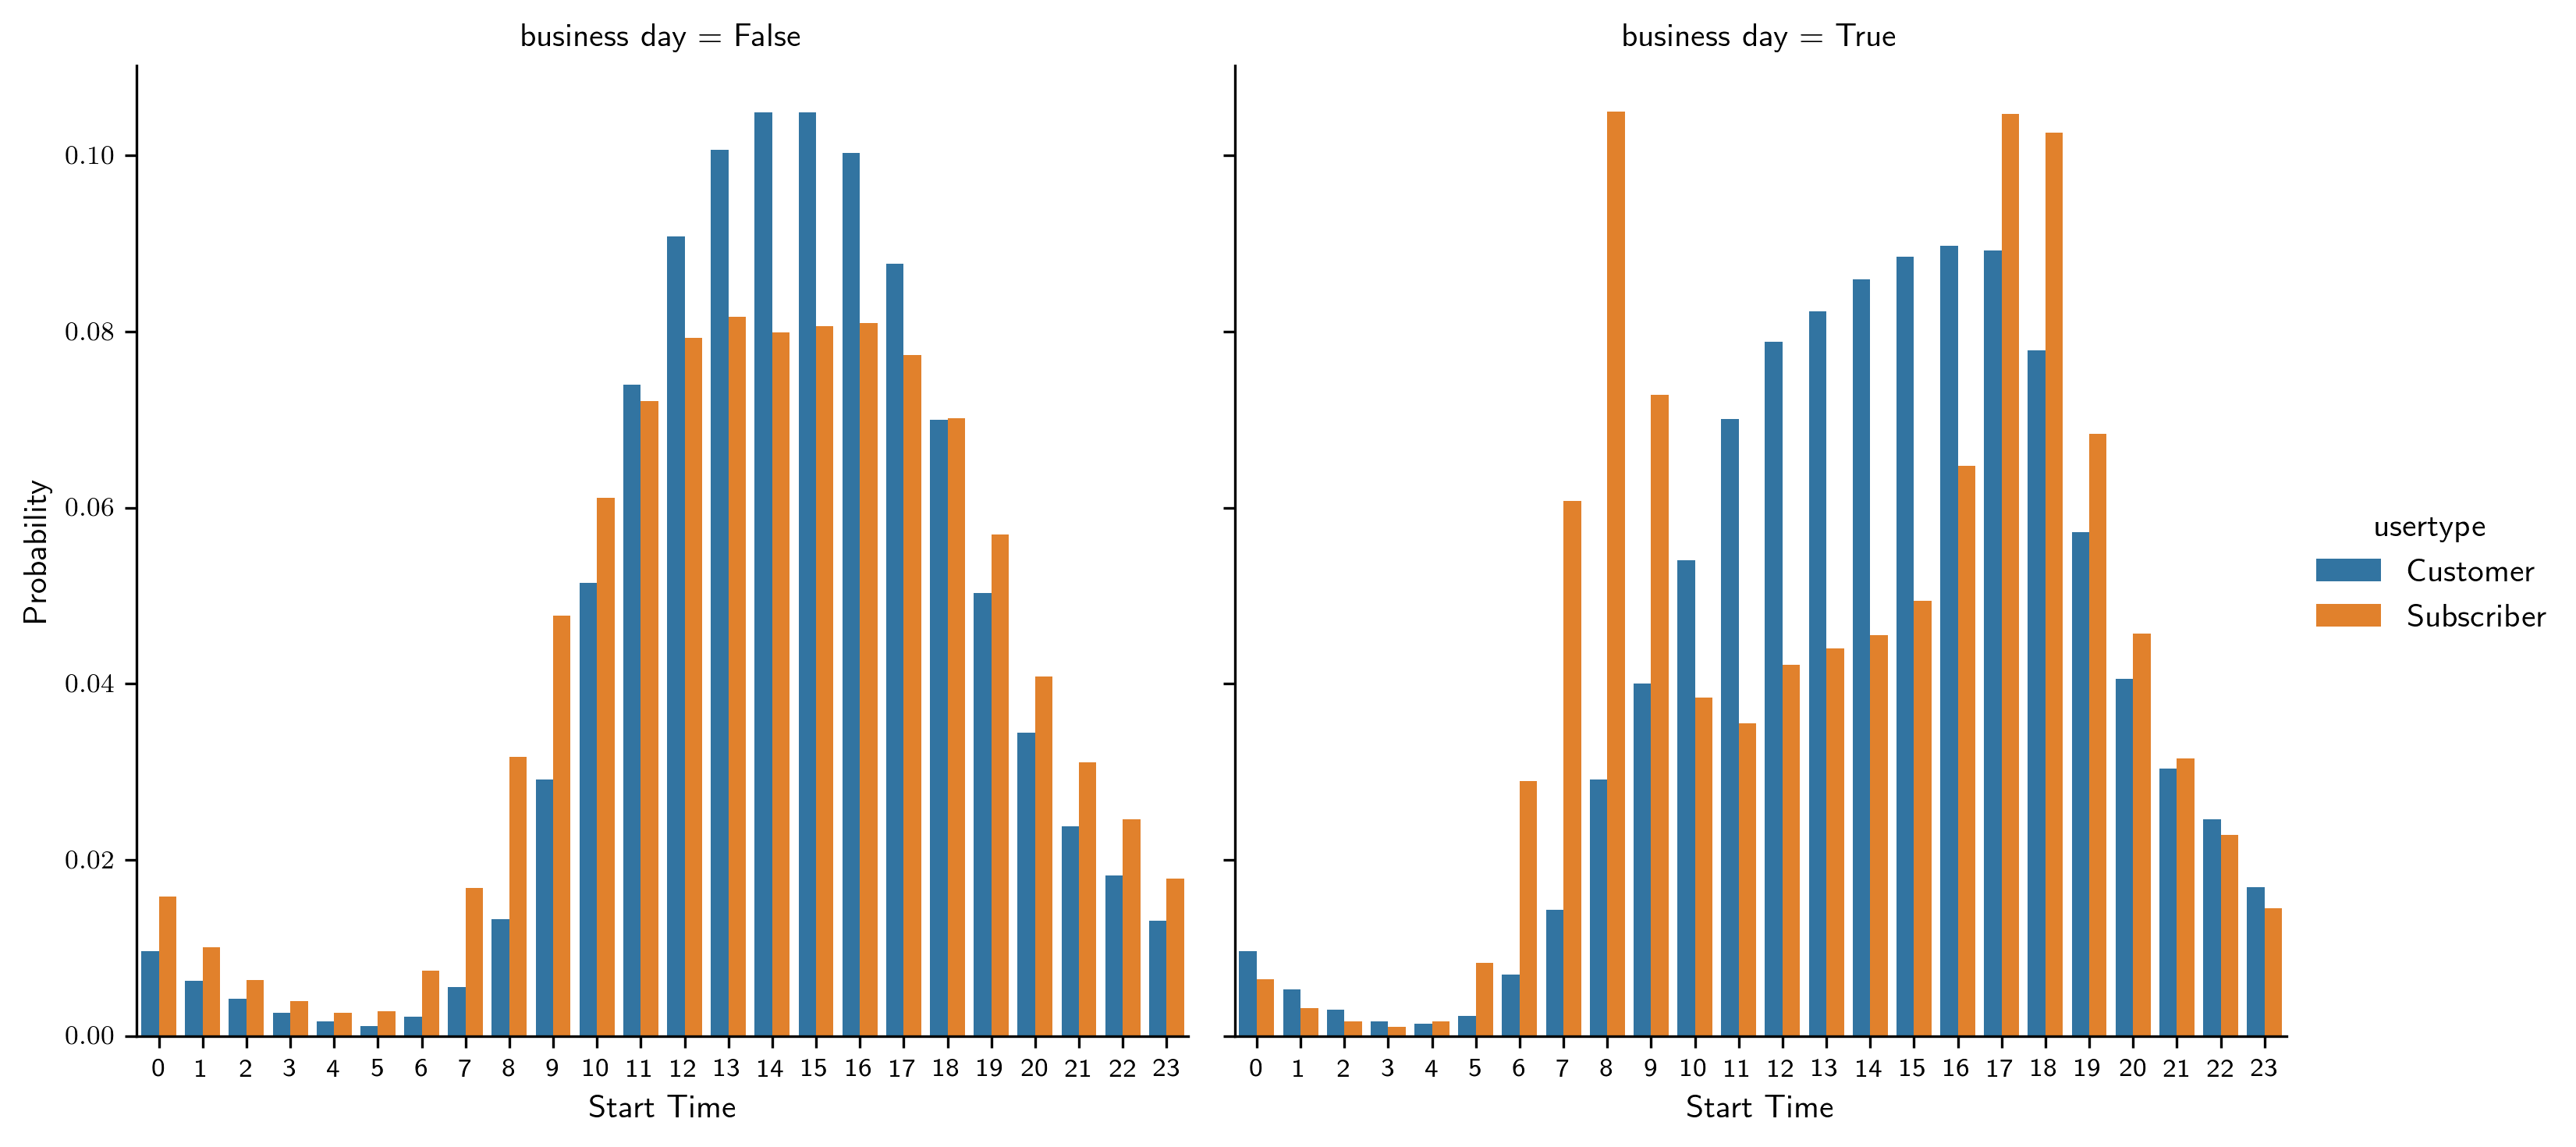
\includegraphics[height=0.6\textheight]{../Images/StartTimeByBusiness}
\myBlock[1]{Zusammenfassung}
{
\begin{itemize}
\item Subscriber nutzen CitiBike auf dem Weg zur Arbeit.
\item Interaktion Werktag x Tageszeit
\end{itemize}
}
\end{frame}

\begin{frame}{Stationen}
\centering
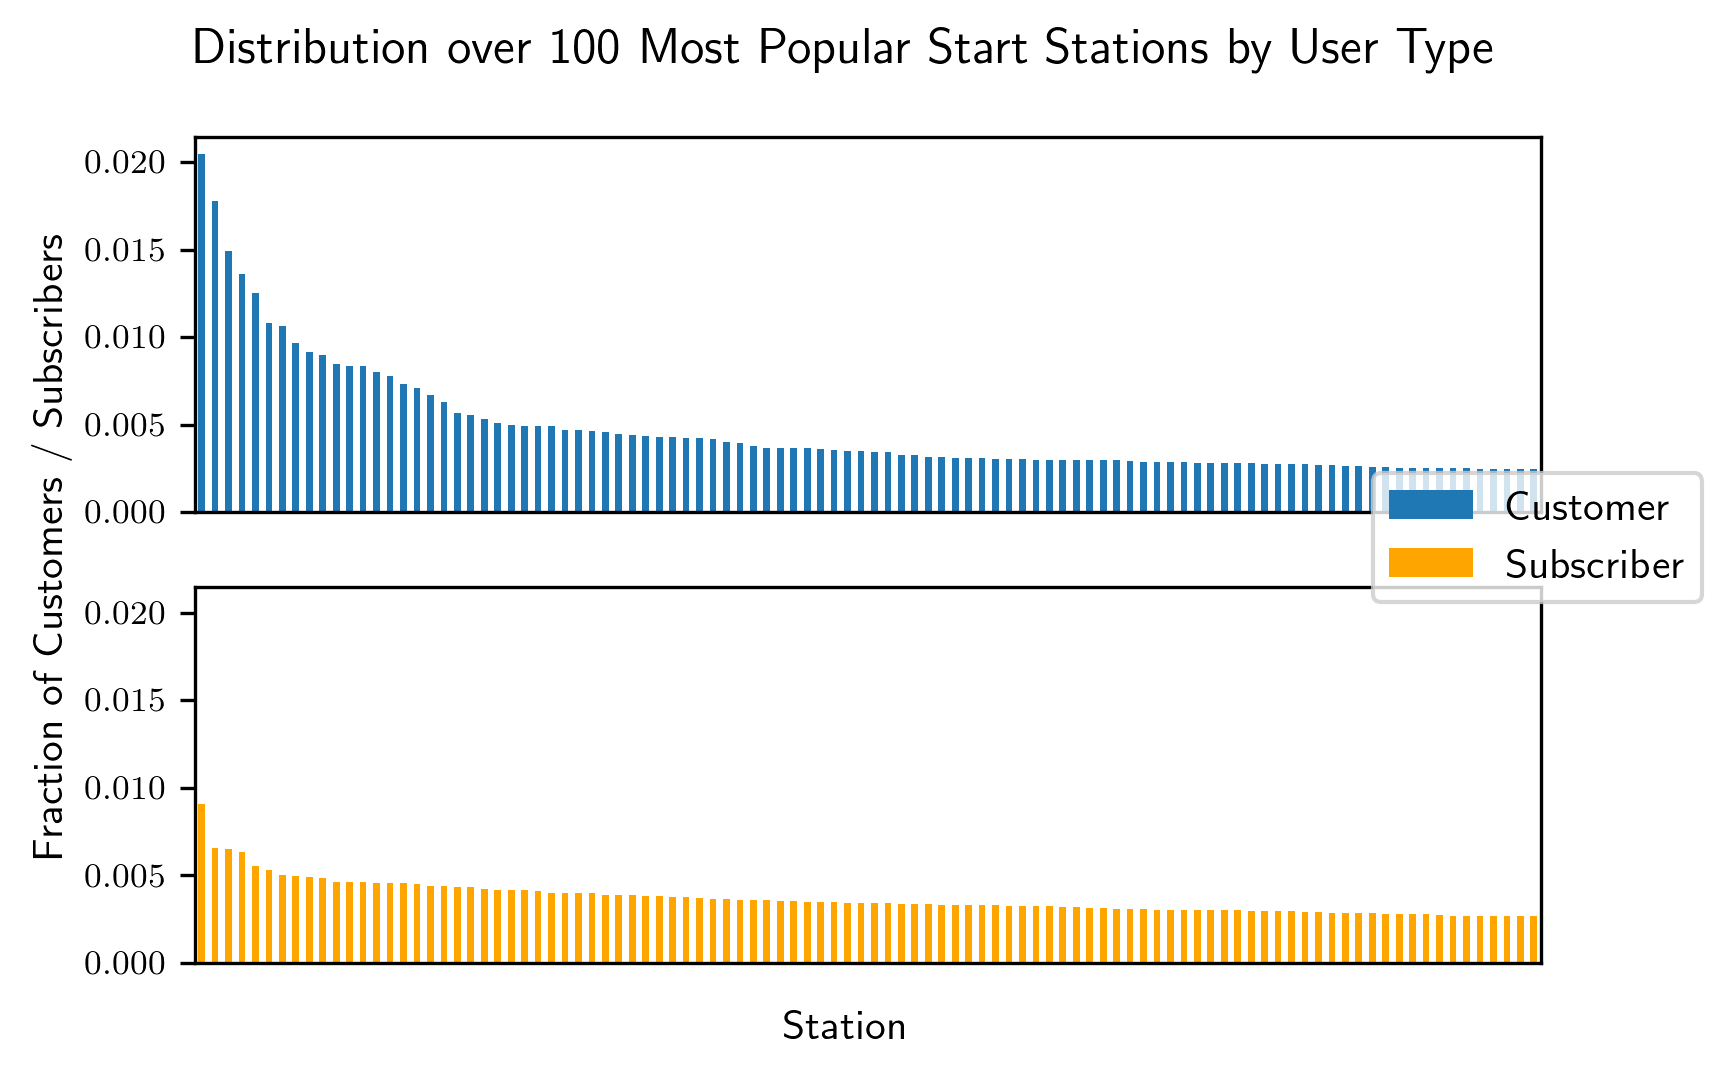
\includegraphics[height=0.6\textheight]{../Images/StartStationPopularity}
\myBlock[1]{Zusammenfassung}
{
\begin{itemize}
\item Customer konzentrieren sich stärker um wenige Stationen.
\item Die 20 beliebtesten Stationen für Customer / Subscriber haben nur 2 gemeinsam.
\item Beliebteste Station Customer: Central Park \hspace{1cm} Subscriber: Pershing Square
\end{itemize}
}
\end{frame}

\begin{frame}{Geschlecht und Alter}
\centering
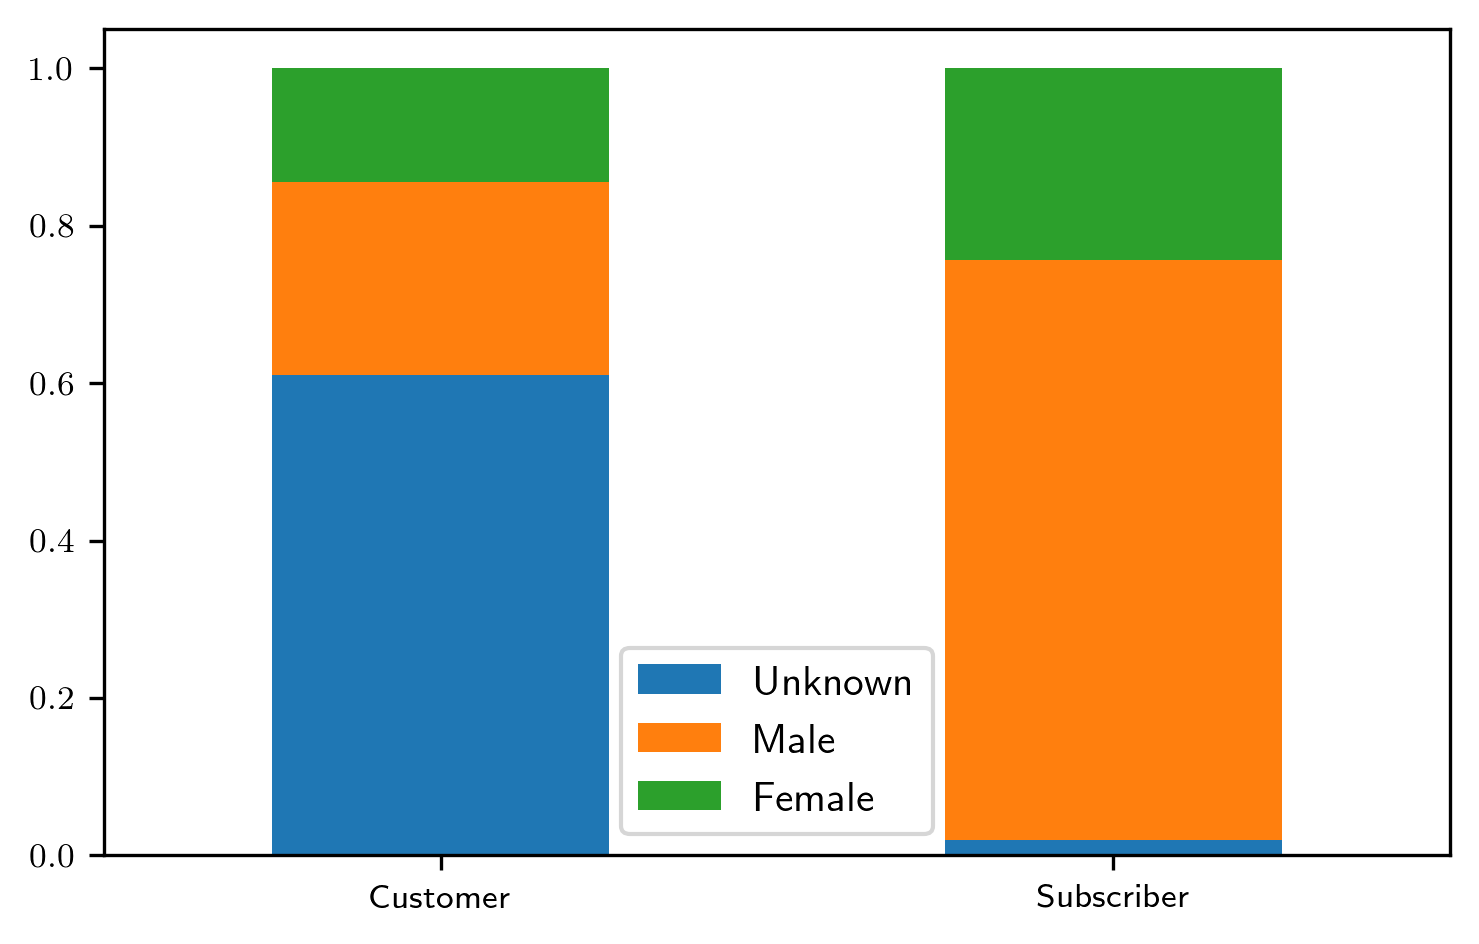
\includegraphics[height=0.5\textheight]{../Images/GenderComparison}
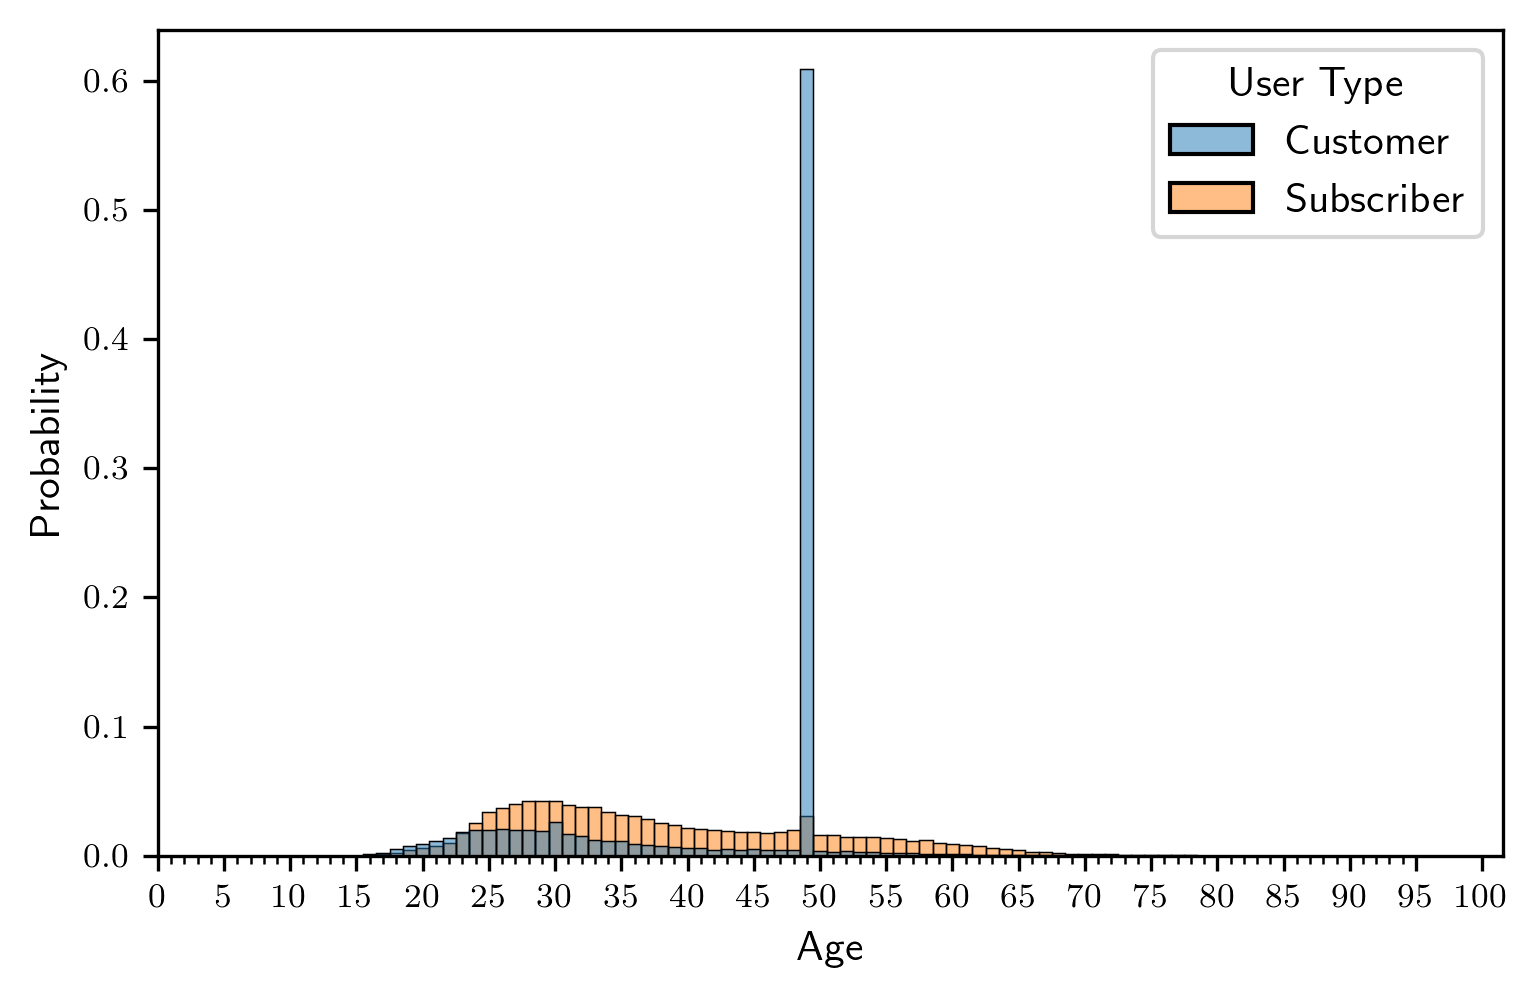
\includegraphics[height=0.5\textheight]{../Images/AgeDistribution}
\myBlock[1]{Zusammenfassung}
{
\begin{itemize}
\item Geschlecht von Customern ist typischerweise unbekannt.
\item Artefakte des Registrierungsprozesses.
\end{itemize}
}
\end{frame}

\begin{frame}
\centering
\myBlock[0.7]{Zusammenfassung}
{
Customer oft Touristen.
\begin{columns}
\begin{column}[t]{0.5\textwidth}
\highlight{Sinnvolle Features}:
\begin{itemize}
\item Sommer/Winter
\item Tageszeit
\item Werktag
\item Distanz
\item Geschwindigkeit
\item Rundfahrt
\item Station
\end{itemize}
\end{column}
\begin{column}[t]{0.5\textwidth}
\highlight{Irreführende Features}:
\begin{itemize}
\item Geschlecht
\item Alter
\end{itemize}
\end{column}
\end{columns}
\vspace{1cm}
}
\end{frame}

\section{Training und Auswahl}

\begin{frame}{Agenda}
\centering
\myBlock[0.6]{}
{
\begin{enumerate}
\item Projektbeschreibung
\item Datenset und Features
\item Feature-Visualisierung
\item \highlight{Modell-Training und -Auswahl}
\item Kooperationsmöglichkeiten mit einer Versicherung
\end{enumerate}
}
\end{frame}

\begin{frame}{Nicht-Balancierte Daten}
\myBlock[0.5]{Evaluierung}
{
\begin{itemize}
\item Baseline-Genauigkeit 89\%
\item Confusion Matrix
\item Matthews Correlation Coefficient (MCC)
\begin{itemize}
\vspace{-1\baselineskip}
\item Korreliert vorhergesagte und echte Klasse.
\item Zwischen -1 und 1, Baseline 0
\item Alle Felder der Confusion Matrix
\end{itemize}
\end{itemize}
}
\myBlock[0.45]{Confusion Matrix}
{
\[
\begin{array}{@{}l*{5}{c}@{}}
\text{Echt} & \multicolumn{2}{c@{}}{\text{Vorhergesagt}}\\
    \cmidrule(l){2-3}
    & \text{Subscriber} & \text{Customer}\\
\midrule
\text{Subscriber} & TN & FN  \\
\text{Customer}   & FP & TP  \\
\bottomrule
\end{array}
\]
\vspace{0.1cm}
}

\myBlock[0.5]{Class-Balancing}
{
\begin{itemize}
\item Gewichtung mit inversem Anteil
\item Implizite Replizierung der seltenen Klasse
\end{itemize}
}
\begin{minipage}{0.4\textwidth}
\centering
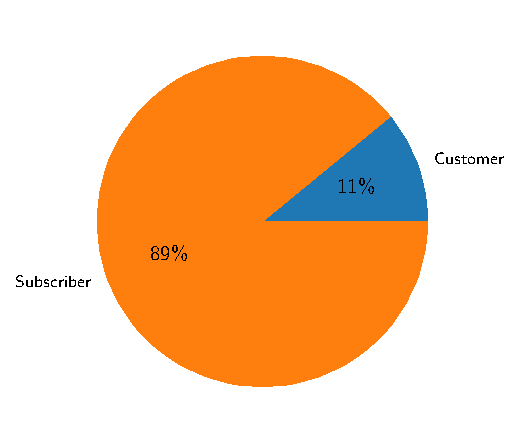
\includegraphics[width=0.8\textwidth]{../Images/Piechart}
\end{minipage}
\end{frame}

\begin{frame}{Logistic Regression}
\myBlock[1]{Modell}
{
\begin{itemize}
\item Lineares Modell für Log-Odds:
\begin{equation}
\log(\frac{p}{1-p}) = X\beta
\end{equation}
\item \highlight{Lineare Decision-Boundary} $x \cdot \beta = 0$.
\item Feature Kodierung sehr relevant.
\item Weight-Decay Regularisierung $\left\lVert\beta\right\rVert_2^2$ $\rightarrow$ Feature-Skalierung relevant.
\item Interaktionen müssen von Hand eingebaut werden.
\item Baseline für andere Modelle.
\end{itemize}
}
\end{frame}

\begin{frame}{Logistic Regression}
\myBlock[1]{Design}
{
\highlight{Features}: Fahrtdauer, Sommer, Werktag, Distanz, Rundfahrt, Geschwindigkeit
\vspace{-0.4cm}
\begin{multicols}{2}
\begin{itemize}
\item Station:
\begin{itemize}
\item Ordinal?
\item Kategorisiert?
\item \highlight{Frequenz kodiert}?
\end{itemize}
\item Tageszeit:
\begin{itemize}
\item Ordinal?
\item \highlight{Kategorisiert}?
\item Zyklisch kodiert?
\end{itemize}
\end{itemize}
\end{multicols}

\highlight{Interaktionen}: Tageszeit x Werktag, Start- x Endstation

\highlight{Skalierung}: Min-Max Skalierung in das Intervall $[0,1]$.

\highlight{Training}: Class-Balancing?
}
\end{frame}

\begin{frame}{Logistic Regression}

\emph{Baseline-Genauigkeit}: 89,1 \%

\begin{columns}
\begin{column}{0.5\textwidth}
\myBlock[1]{Ohne Class-Balancing}
{
\begin{itemize}
\item \highlight{Genauigkeit: 90,4 \%}
\item Confusion:
%Table from https://tex.stackexchange.com/questions/339535/what-to-put-into-the-intersection-of-the-row-column-labels-of-a-table
\[
\begin{array}{@{}l*{5}{c}@{}}
\text{Echt} & \multicolumn{2}{c@{}}{\text{Vorhergesagt}}\\
    \cmidrule(l){2-3}
    & \text{Subscriber} & \text{Customer}\\
\midrule
\text{Subscriber} & 98,2\% & 1,8 \% \\
\text{Customer}   & 72,7 \% & 27,3 \% \\
\bottomrule
\end{array}
\]
\item MCC: $0,38$
\end{itemize}
}
\end{column}
\begin{column}{0.5\textwidth}
\myBlock[1]{Mit Class-Balancing}
{
\begin{itemize}
\item Genauigkeit: 79,5 \%
\item Confusion:
%Table from https://tex.stackexchange.com/questions/339535/what-to-put-into-the-intersection-of-the-row-column-labels-of-a-table
\[
\begin{array}{@{}l*{5}{c}@{}}
\text{Echt} & \multicolumn{2}{c@{}}{\text{Vorhergesagt}}\\
    \cmidrule(l){2-3}
    & \text{Subscriber} & \text{Customer}\\
\midrule
\text{Subscriber} & 79,6\% & 20,4 \% \\
\text{Customer}   & 21,7 \% & \highlight{78,3 \%} \\
\bottomrule
\end{array}
\]
\item MCC: $0,41$
\end{itemize}
}
\end{column}
\end{columns}

\myBlock[1]{Wichtige Features}
{
Fahrtdauer, Distanz, Geschwindigkeit, Stationen
}
\end{frame}

\begin{frame}{Decision-Tree und Random-Forest}
\myBlock[1]{Decision Tree}
{
\begin{itemize}
\item Serie von Splits des Datensets.
\item Nicht-Lineares Modell.
\item Findet Interaktionen.
\item \highlight{Tendiert zu Overfitting}.
\end{itemize}
}
\myBlock[1]{Random-Forest}
{
\begin{itemize}
\item Bagging mehrerer Decision-Trees.
\item Bootstrap-Sampling der Training-Daten.
\item Zufällige Maskierung von Features in jedem Split.
\item Kontrolliert Overfitting.
\end{itemize}
}
\end{frame}

\begin{frame}{Decision-Tree}
\myBlock[1]{Design}
{
\begin{itemize}
\item Feature-Kodierung und -Skalierung weniger relevant.
\item Class-Balancing
\item Mehrere Hyperparameter, z.B.: Maximale Tiefe, Anzahl Bäume
\end{itemize}
}
%\begin{columns}
%\begin{column}{0.4\textwidth}
\centering
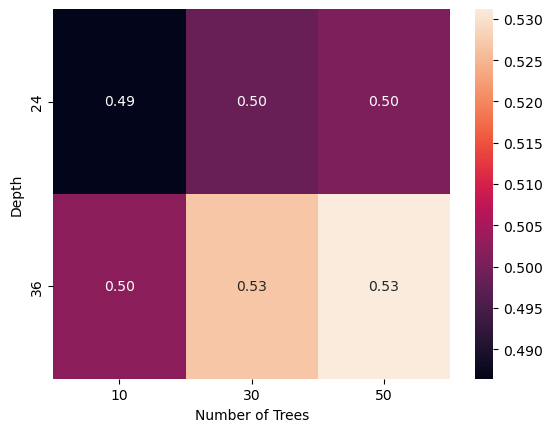
\includegraphics[width=0.48\textwidth]{Bilder/GridSearchMCC} 
%\end{column}
%\begin{column}{0.6\textwidth}
%\myBlock[1]{Ergebnisse}
%{
%\begin{itemize}
%\item MCC: Forest $>$ Tree $>$ Regression.
%\item Kleinere Bäume und Logistic Regression haben höhere Genauigkeit auf Customers (vermeiden Overfitting).
%\end{itemize}
%}
%\end{column}
%\end{columns}
\end{frame}

\begin{frame}{Finale Auswertung}

\myBlock[1]{Performance-Vorhersage}
{
\makebox[2cm][l]{\highlight{Training}:} Auf Training + Validation Set

\makebox[2cm][l]{\highlight{Evaluation}:} Auf Test Set
}

\begin{columns}
\begin{column}{0.5\textwidth}
\myBlock[1]{Forest}
{
\highlight{Insgesamt bestes Modell}.
\begin{itemize}
\item \highlight{Genauigkeit: 91,8 \%}
\item Confusion:
%Table from https://tex.stackexchange.com/questions/339535/what-to-put-into-the-intersection-of-the-row-column-labels-of-a-table
\[
\begin{array}{@{}l*{5}{c}@{}}
\text{Echt} & \multicolumn{2}{c@{}}{\text{Vorhergesagt}}\\
    \cmidrule(l){2-3}
    & \text{Subscriber} & \text{Customer}\\
\midrule
\text{Subscriber} & 97,2 \% & 2,8 \% \\
\text{Customer}   & 51,2 \% & 48,7 \% \\
\bottomrule
\end{array}
\]
\item \highlight{MCC: $0,53$}
\end{itemize}
}
\end{column}
\begin{column}{0.5\textwidth}
\myBlock[1]{Decision-Tree}
{
\highlight{Hohe Genauigkeit auf Customers}.
\begin{itemize}
\item Genauigkeit: 82,9 \%
\item Confusion:
%Table from https://tex.stackexchange.com/questions/339535/what-to-put-into-the-intersection-of-the-row-column-labels-of-a-table
\[
\begin{array}{@{}l*{5}{c}@{}}
\text{Echt} & \multicolumn{2}{c@{}}{\text{Vorhergesagt}}\\
    \cmidrule(l){2-3}
    & \text{Subscriber} & \text{Customer}\\
\midrule
\text{Subscriber} & 84,2 \% & 15,8 \% \\
\text{Customer}   & 28,1 \% & \highlight{71,9 \%} \\
\bottomrule
\end{array}
\]
\item MCC: $0,42$
\end{itemize}
}
\end{column}
\end{columns}
\end{frame}

\begin{frame}
\centering
\myBlock[0.8]{Zusammenfassung}
{
\begin{itemize}
\item Modell Wahl hängt vom Anwendungsfall ab.
\item \highlight{Insgesamt bestes Modell} (MCC):

 Großer Random-Forest

\item Klares Overfitting vor allem auf Customers, Verbesserung durch mehr Trees oder Pruning? 
 
\item \highlight{Hohe Genauigkeit auf Customers}:

Kleinerer Decision-Tree/Logistic Regression
\item Hohe Genauigkeit auf Customers z.B.\ relevant im Marketing.
\end{itemize}
}
\end{frame}

\section{Kooperation mit einer Versicherung}

\begin{frame}{Agenda}
\centering
\myBlock[0.6]{}
{
\begin{enumerate}
\item Projektbeschreibung
\item Datenset und Features
\item Feature-Visualisierung
\item Modell-Training und -Auswahl
\item \highlight{Kooperationsmöglichkeiten mit einer Versicherung}
\end{enumerate}
}
\end{frame}

\begin{frame}{Kooperation mit einer Versicherung}
\myBlock[1]{Analyse der Unfallstatistik des NYPD}
{
\begin{itemize}
\item Radfahrer haben 4-5 mal weniger Unfälle als Taxis.
\item Die Rate an Verletzungen pro Fahrt ist ebenfalls etwas niedriger.
\item Bei einem Fahrradunfall wird in ca. 70\% der Fälle ein Radfahrer verletzt.
\item Bei ca.\ 40\% der Unfälle mit Fahrrädern hatte der Fahrradfahrer einen Beitrag.
\item Bei ca.\ 2\% der Unfälle mit Fahrrädern hatte das Fahrrad einen Defekt.
\end{itemize}
}
\myBlock[1]{Kooperationsmöglichkeiten}
{
CitiBike übernimmt bei einem Unfall keine Kosten, außer bei defekten Rädern.
\begin{itemize}
\item Unfallversicherung für Nutzer (häufige Personenschäden).
\begin{itemize}
\item Viele Fahrten allerdings auf dem Arbeitsweg.
\end{itemize}
\item Haftpflichtversicherung für Nutzer (häufige Mitschuld).
\item Versicherung des Verleihers im Fall defekter Räder (selten).
\item Rabatte bei Versicherungen für Subscriber.
\end{itemize}
}
\end{frame}

\begin{frame}{Decision Tree and Random Forest}
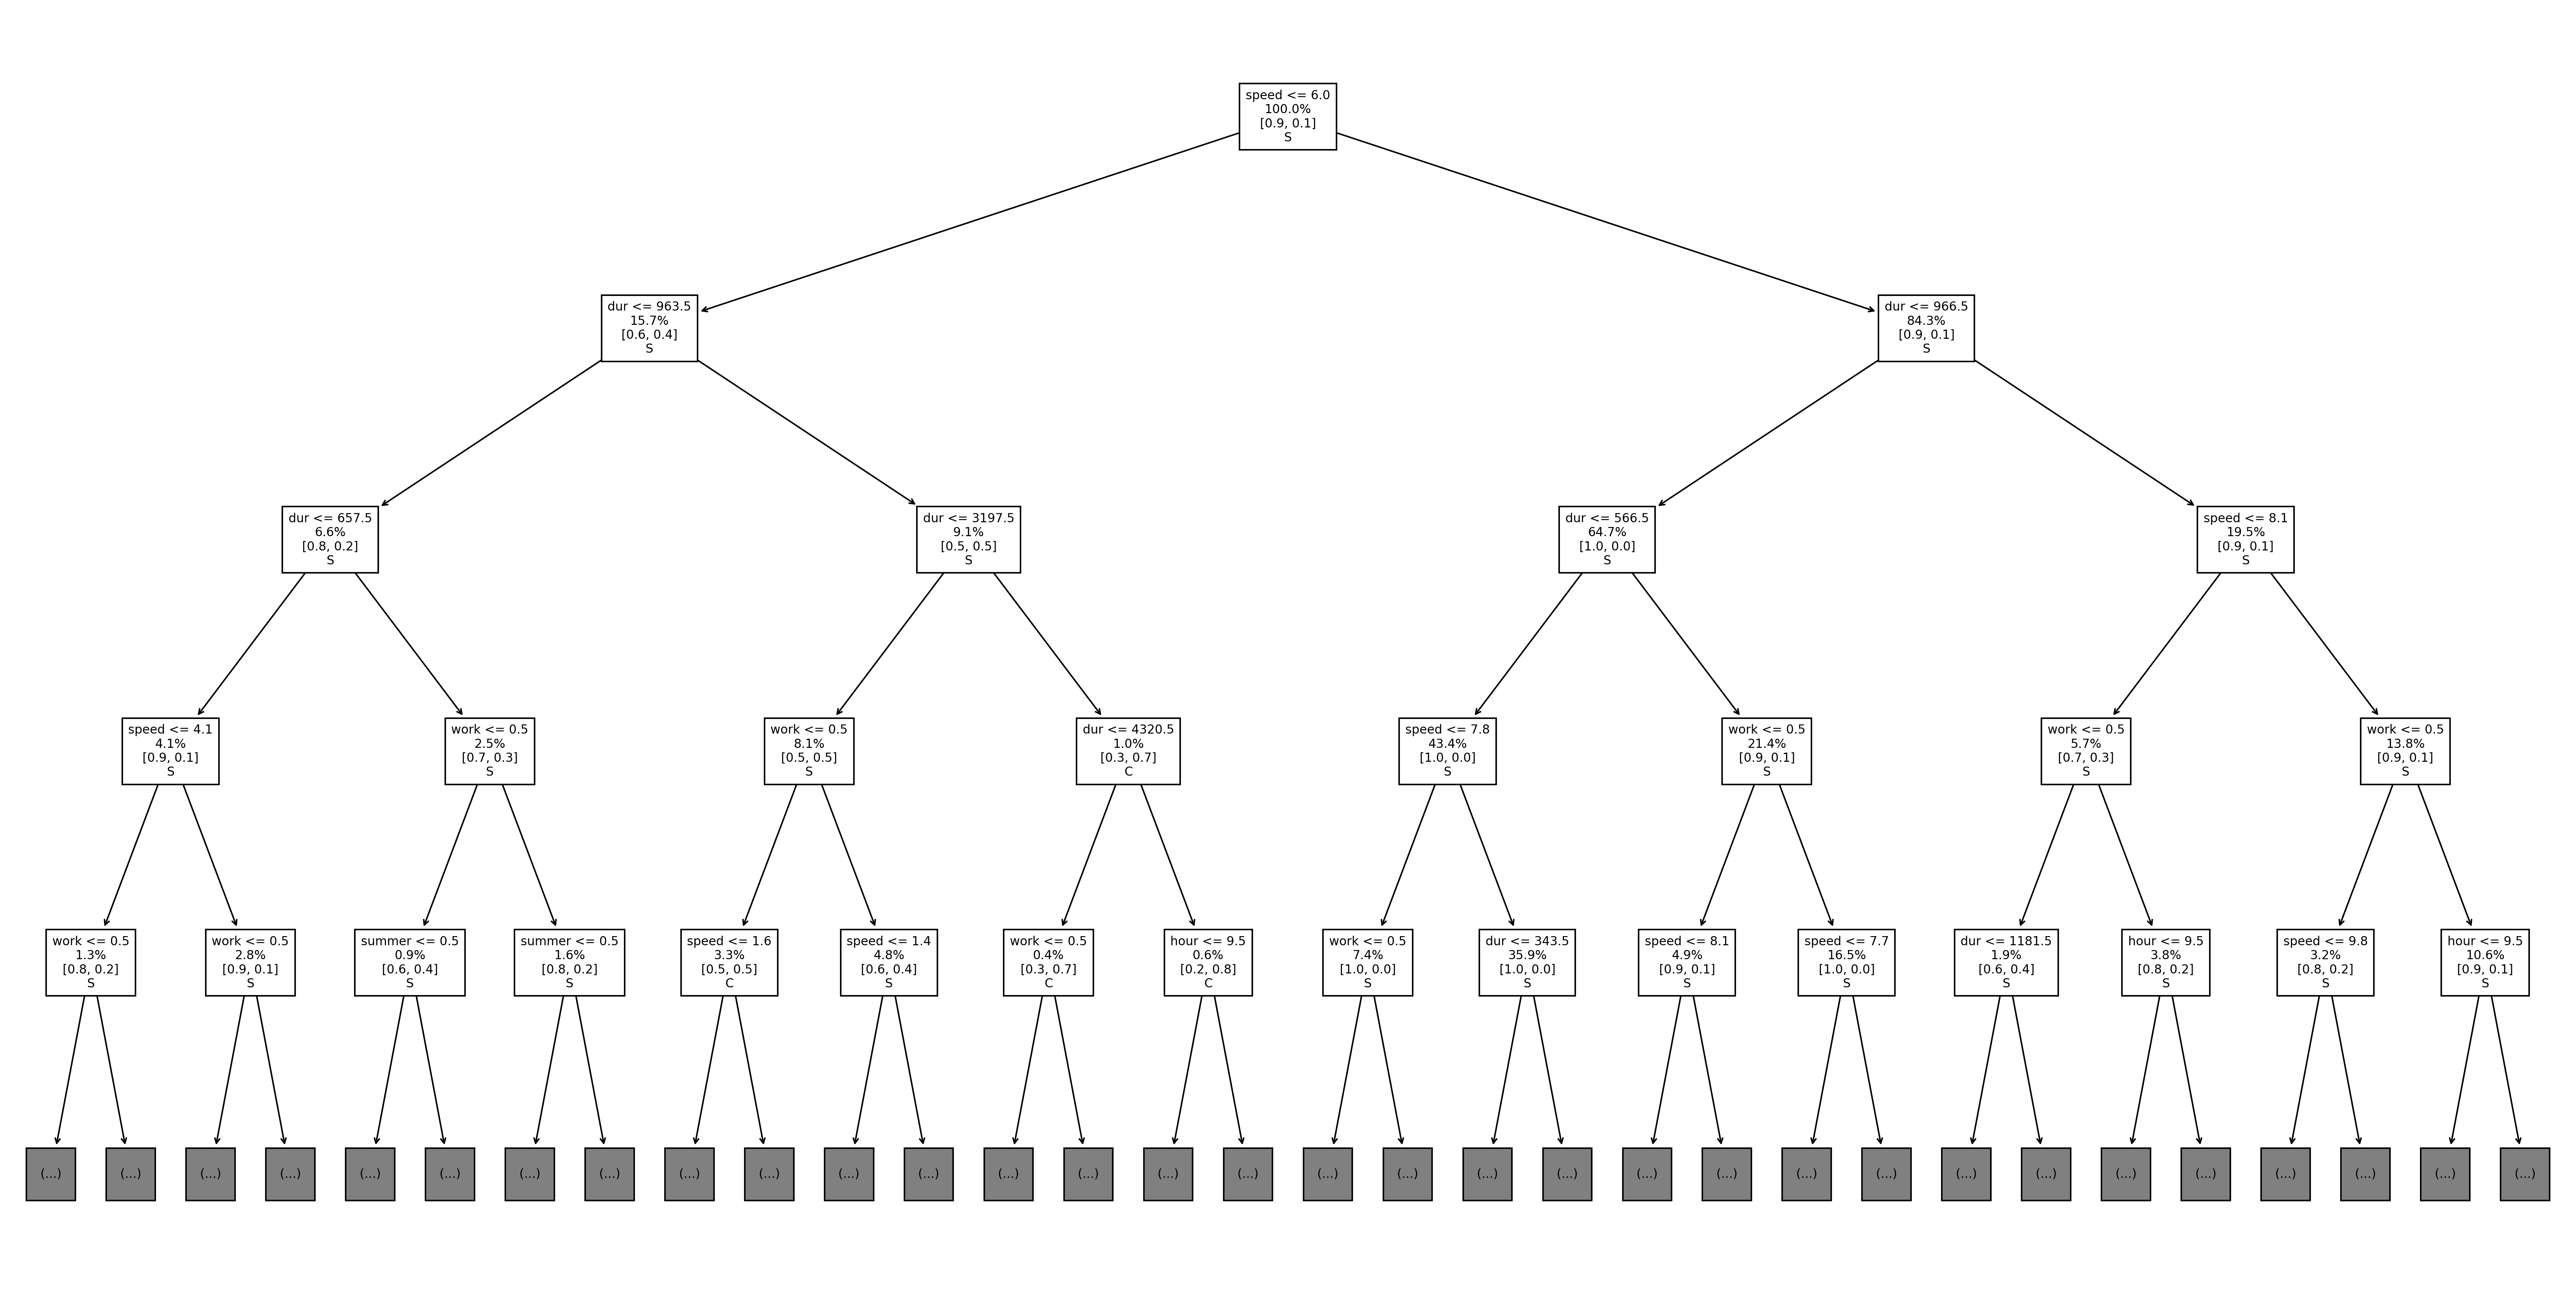
\includegraphics[width=\textwidth]{../Images/ExampleTree}
\end{frame}






%%% -------------------------------------
\end{document}